\chapter[Introdução]{Introdução}

% TRECHO ALTERADO PARA EXPLICAR O PORQUE DA IMPORTÂNCIA DE AVALIAR A DOR
A identificação e quantificação da dor em animais permanecem como desafios centrais na pesquisa experimental, apresentando implicações diretas para o bem-estar animal, a ética científica e a confiabilidade dos resultados obtidos. Quando não reconhecida ou subestimada, a dor pode ocasionar sofrimento desnecessário, além de desencadear alterações fisiológicas e comportamentais duradouras, como processos de sensibilização do sistema nervoso central, incluindo quadros de hiperalgesia — caracterizados pelo aumento da sensibilidade a estímulos dolorosos — bem como alterações no comportamento social dos animais. Como consequência, a dor passa a atuar como uma variável de confusão, comprometendo a validade interna dos estudos, reduzindo sua reprodutibilidade e dificultando a correta interpretação dos resultados obtidos. \cite{turner2019pain, Carbone2011, sneddon2014}. 

Em um contexto experimental, os camundongos destacam-se como um dos modelos vertebrados mais utilizados para pesquisas biomédicas, em áreas como genética, fisiologia e medicina. Isto está associado à fatores como a elevada similaridade genética com os seres humanos, a facilidade de manejo em ambientes controlados e o ciclo de vida favorável, caracterizado por curto período de gestação e rápida maturidade sexual \cite{chorilli2007}.

% TRECHO NOVO PARA DESTACAR A ATUAÇÃO DO PROFISSIONAL
Durante a condução de experimentos envolvendo modelos animais, espera-se que os pesquisadores realizem monitoramento contínuo das condições clínicas dos indivíduos, identificando precocemente sinais compatíveis com dor ou sofrimento, buscando subsidiar decisões relacionadas à administração de analgésicos, à necessidade de refinamento dos procedimentos experimentais e, em situações críticas, à interrupção ética do experimento \cite{NRC2011Guide}.

A avaliação de dor em camundongos — assim como em outras espécies animais — apresenta desafios intrínsecos decorrentes da incapacidade destes animais em verbalizar suas sensações. Dessa forma, o processo ainda é fortemente dependente da interpretação e expertise do avaliador, o que pode ocasionar um certo grau de viés às análises. Nesse sentido, a participação — ou ao menos a supervisão — de profissionais qualificados, como médicos-veterinários e especialistas em bem-estar animal, é considerada essencial para garantir tanto a qualidade científica quanto a adoção de boas práticas experimentais \cite{concea2019}.

% TRECHO NOVO PARA EXPLICAR AS LIMITAÇÕES NO CENÁRIO PRÁTICO
No Brasil, estudos envolvendo indução de dor são submetidos à aprovação das Comissões de Ética no Uso de Animais (CEUA), que verificam a justificativa científica do modelo, o monitoramento do bem-estar animal e a capacitação da equipe executora, conforme as diretrizes do CONCEA e a Lei nº 11.794/2008. Embora a legislação não determine que tais avaliações sejam realizadas exclusivamente por médicos-veterinários, exige que os procedimentos sejam conduzidos por pessoal qualificado e que haja supervisão e assistência veterinária para assegurar o bem-estar dos animais. Em protocolos que envolvem grande número de animais e avaliações seriadas ao longo do tempo, a necessidade de observadores treinados pode representar um desafio operacional, aumentando a carga de trabalho, dificultando a padronização entre avaliadores, o que potencialmente impacta a consistência e a reprodutibilidade dos resultados experimentais.\cite{Colby2007, concea2019}.

Buscando reduzir a subjetividade na avaliação humana e minimizar a dependência da mão de obra altamente especializada, diferentes metodologias baseadas em indicadores comportamentais foram propostas ao longo dos anos. Dentre elas, destaca-se a \textit{Grimace Scale}, uma escala destinada à mensuração da dor por meio de alterações nas expressões faciais dos animais. Em particular, a \textit{Mouse Grimace Scale} (\acs{MGS}) avalia modificações em cinco regiões faciais distintas em camundongos — orelhas, olhos, bochechas, nariz e bigodes — que apresentam alterações características em resposta a estímulos dolorosos, conforme ilustrado na Figura \ref{fig:mgs_indicators}.

\begin{figure}[h]
	\centering
	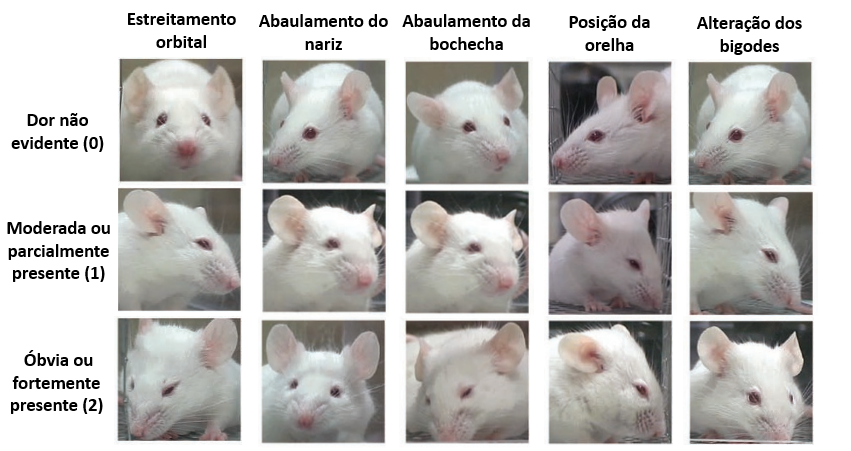
\includegraphics[width=1\linewidth]{figuras/figs_introducao/MGS.png}
	\caption{Indicadores da \acs{MGS} utilizados para a avaliação da dor em camundongos. A figura apresenta cinco unidades de expressões faciais: estreitamento orbital, protrusão nasal, protrusão das bochechas, posição das orelhas e alteração nos bigodes. Para cada característica, são mostrados exemplos representativos correspondentes à três níveis de intensidade: 0 (ausente), 1 (moderado) e 2 (grave). Fonte: Adaptado de \cite{Langford2010}.}
	\label{fig:mgs_indicators}
\end{figure}

A principal contribuição da \acs{MGS} consiste na padronização das análises conduzidas em ambientes experimentais, por meio da definição objetiva das unidades de expressão facial e dos critérios necessários para sua classificação. Entretanto, a avaliação ainda depende da interpretação humana, exigindo avaliadores devidamente treinados para identificar e classificar os indicadores de forma consistente. Em estudos que envolvem grande número de animais ou avaliações seriadas, essa dependência ainda pode representar um desafio operacional.

Diante dessas limitações, técnicas automatizadas baseadas em visão computacional e aprendizado de máquina têm emergido como alternativas promissoras para a avaliação da dor, apresentando potencial para reduzir possíveis vieses humanos e viabilizar avaliações mais ágeis, consistentes e reprodutíveis no contexto da pesquisa com modelos animais \cite{Zamzmi2019}.

Portanto, o presente trabalho propõe o desenvolvimento de um modelo baseado em visão computacional e aprendizado de máquina voltado à identificação automática dos marcadores definidos pela \acs{MGS}, seguido da classificação quanto à presença e intensidade da dor. Além de reduzir a dependência de técnicas manuais de extração de características, o estudo busca ampliar a aplicabilidade das soluções propostas em cenários experimentais próximos de condições reais. Adicionalmente, são investigadas diferentes arquiteturas de redes neurais, analisando o impacto de fatores estruturais — como profundidade das redes, regimes de treinamento e configurações de hiperparâmetros — sobre o desempenho dos modelos.

\section{Motivação}

% SEÇÃO ALTERADA PARA DAR MAIOR IMPORTANCIA AO MEU TRABALHO 
Além das contribuições para a área de visão computacional, ferramentas automatizadas para avaliação da dor apresentam potencial para apoiar médicos-veterinários e pesquisadores durante o monitoramento de animais submetidos a protocolos experimentais. O fornecimento de estimativas objetivas sobre a presença e a intensidade da dor contribuem para decisões relacionadas à administração de analgesia, ao refinamento dos protocolos experimentais e à definição de intervenções clínicas quando necessárias. 

Nesse contexto, a disponibilidade de ferramentas capazes de fornecer avaliações padronizadas da dor também favorece a uniformização das condutas adotadas entre diferentes profissionais e instituições. A redução da variabilidade entre avaliadores contribui para decisões clínicas mais consistentes, além de fortalecer a comparabilidade dos resultados obtidos em estudos e experimentos conduzidos por diferentes grupos de pesquisa.

Por fim, além de automatizar um processo de classificação de imagens, a proposta deste trabalho busca disponibilizar uma ferramenta de apoio à tomada de decisão por médicos-veterinários e pesquisadores, favorecendo a adoção de práticas experimentais mais éticas, padronizadas e reprodutíveis, em conformidade com os princípios contemporâneos de bem-estar animal e refinamento experimental. Dessa forma, a tecnologia proposta deve ser compreendida como um instrumento de complementar — e não substitutivo — do processo de avaliação realizada por profissionais especializados.

\section{Objetivos}

O principal objetivo deste trabalho consiste no desenvolvimento e na avaliação de um sistema baseado em visão computacional e aprendizado de máquina para auxiliar a identificação e a classificação automática da presença e da intensidade da dor em camundongos, utilizando os parâmetros estabelecidos pela \acs{MGS}. Espera-se que a ferramenta desenvolvida contribua para avaliações mais objetivas, padronizadas e reprodutíveis, oferecendo suporte à tomada de decisão por pesquisadores e médicos-veterinários durante o monitoramento de animais utilizados em pesquisas biomédicas. Adicionalmente, o estudo busca investigar diferentes abordagens de classificação baseadas em redes neurais, visando identificar as arquiteturas e configurações mais adequadas para o problema proposto. A partir dessa premissa, o trabalho desdobra-se nos seguintes objetivos específicos:

\begin{enumerate}
	
	\item Realizar um levantamento do estado da arte sobre métodos computacionais aplicados à detecção e classificação de padrões em dados de imagens;
	
	\item Especificar os equipamentos e protocolos empregados na aquisição das imagens utilizadas no estudo;
	
    \item Desenvolver uma ferramenta computacional destinada à extração, organização e gerenciamento das imagens utilizadas na construção da base de dados;
    
    \item Realizar o tratamento das imagens coletadas, adequando-as para as etapas de treinamento e validação dos classificadores;

	\item Implementar os modelos neurais responsáveis pelas classificação dos padrões faciais associados à dor, de acordo com a \acs{MGS};
	
	\item Treinar e avaliar os modelos implementados, utilizando métricas adequadas de desempenho;
	
	\item Realizar uma análise comparativa entre os modelos investigados, buscando identificar as arquiteturas mais otimizadas para o problema proposto;
	
	\item Investigar o impacto de diferentes configurações de hiperparâmetros e estratégias de treinamento sobre o desempenho dos modelos.
	
	%\item Analisar as implicações práticas da utilização de sistemas automatizados para detecção de dor em contextos experimentais e veterinários.
    
\end{enumerate}

\section{Hipótese}

A hipótese central deste estudo é que modelos neurais aplicados à visão computacional sejam capazes de identificar automaticamente os indicadores estabelecidos pela \acs{MGS} em imagens das regiões faciais de camundongos, possibilitando a detecção e a quantificação da dor.

Parte-se do pressuposto de que a extração automatizada e padronizada de características visuais possibilite a identificação de nuances associadas aos indicadores da \acs{MGS}, inclusive padrões sutis que dificilmente seriam detectados por observadores não especializados.

\section{Revisão do Estado da Arte}

O problema da identificação e quantificação da dor não é recente, porém ainda apresenta desafios e limitações significativos, os quais motivam o desenvolvimento de novas técnicas e abordagens para sua análise. Nesse contexto, os avanços recentes em visão computacional e aprendizado de máquina têm impulsionado diferentes estudos voltados à identificação e classificação automática de sinais associados à dor em diferentes espécies animais.

% CITAÇÃO AO TUTTLE ALTERADA PARA DIFERENCIAR MELHOR DESTA PESQUISA
O estudo desenvolvido por \cite{Tuttle2018DNNPain} representa um dos primeiros trabalhos a investigar a aplicação de aprendizado profundo para automatizar a \acs{MGS}. Os autores propuseram um sistema baseado na arquitetura convolucional InceptionV3, treinado com aproximadamente 5.700 imagens previamente rotuladas por especialistas, cujo objetivo consistiu em substituir a pontuação manual realizada por avaliadores humanos. O modelo realizou uma classificação binária entre presença e ausência de dor, alcançando aproximadamente 94\% de acurácia e elevada correlação com as avaliações humanas.

Embora esse estudo tenha demonstrado a viabilidade da automatização da MGS, sua investigação concentrou-se na validação de uma única arquitetura convolucional e em um cenário específico de classificação binária. Aspectos relacionados ao impacto de diferentes arquiteturas neurais, estratégias de treinamento, configurações de hiperparâmetros e modelos baseados em mecanismos de atenção não foram explorados. Em contraste, o presente trabalho adota uma perspectiva mais ampla ao investigar comparativamente diferentes modelos de aprendizado profundo. Dessa forma, além de propor uma solução computacional, esta pesquisa busca compreender quais abordagens apresentam maior potencial para o problema proposto.

Outra contribuição relevante foi apresentada por \cite{Wotton2020}, que desenvolveram um sistema automatizado de fenotipagem comportamental aplicado ao teste da formalina em camundongos. O estudo teve como objetivo automatizar a identificação de comportamentos nociceptivos — como lamber, morder e elevar a pata — sem depender de observação humana contínua. Diferentemente da abordagem baseada na \acs{MGS}, o trabalho concentrou-se em padrões comportamentais corporais, e não exclusivamente em expressões faciais.

A metodologia proposta foi estruturada em três etapas principais. Inicialmente, foi feita a detecção de pontos-chave corporais por meio do \textit{DeepLabCut}, ferramenta baseada em \acsp{CNN} com arquitetura \textit{ResNet}-50. Em seguida, foram extraídas características espaço-temporais utilizando distâncias euclidianas e ângulos entre pontos anatômicos ao longo das sequências temporais. Por fim, os comportamentos nociceptivos foram classificados utilizando o algoritmo \textit{GentleBoost}, baseado em conjuntos de árvores de decisão. O sistema alcançou concordância de 98\% em relação às avaliações humanas.

Abordagens semelhantes também têm sido aplicadas em outras espécies animais. No contexto veterinário, \cite{lencioni2021} investigaram a detecção automática de dor em equinos por meio da análise de expressões faciais indicadas pela \textit{Grimace Scale}. O sistema desenvolvido utilizou \acsp{CNN} independentes para analisar diferentes regiões da face — incluindo orelhas, olhos e boca/narinas — cujas saídas foram posteriormente integradas em um classificador global responsável pela decisão final. Os resultados indicaram que o modelo dedicado à análise das orelhas apresentou o melhor desempenho individual, alcançando acurácia de 90,3\%. Já os modelos associados às regiões dos olhos e boca/narinas obtiveram acurácias de 65,5\% e 74,5\%, respectivamente. Na classificação global, o sistema atingiu acurácia de 75,8\%. Contudo, quando a tarefa foi simplificada para classificação binária entre presença e ausência de dor, o valor de acurácia subiu para 88,3\%.

Além das aplicações veterinárias, métodos automatizados de detecção da dor também vêm sendo investigados no contexto humano. O trabalho descrito por \cite{karamitsos2021} propõe uma abordagem baseada em \acsp{CNN} para monitoramento automático da dor em pacientes clínicos por meio de expressões faciais, visando aplicações em sistemas hospitalares de monitoramento contínuo. O estudo utilizou a base de dados \textit{UNBC-McMaster Shoulder Pain Expression Archive}, amplamente empregada na literatura para tarefas de reconhecimento de expressões faciais associadas à dor. Após as etapas de pré-processamento, as imagens foram utilizadas no treinamento de uma versão adaptada da arquitetura \textit{\acs{VGG}16} para a indicação da presença ou ausência de dor.

Os resultados deste estudo demonstraram acurácia de 92,5\% e \textit{recall} de 86,96\% no conjunto de teste, superando abordagens previamente reportadas na literatura, incluindo modelos híbridos e arquiteturas recorrentes. Apesar do desempenho satisfatório, os autores destacaram limitações relacionadas ao desbalanceamento das classes e à necessidade de ampliar a diversidade do conjunto de treinamento, com enfoque no desenvolvimento de estratégias futuras voltadas à redução de falsos positivos.

É importante destacar que os estudos supracitados compartilham uma característica comum: o uso predominante de modelos neurais convolucionais. Os quais foram especificamente projetados para processamento de dados com estrutura espacial, -- como imagens -- e consolidaram-se na literatura devido a capacidade de realizar extração automática de características relevantes, além da elevada eficiência observada em tarefas de visão computacional. Entretanto, apesar dos avanços proporcionados pelas \acsp{CNN}, tais arquiteturas apresentam limitações relacionadas à modelagem de dependências globais na imagem, uma vez que operam predominantemente sobre padrões locais extraídos por convoluções sucessivas. Nesse cenário, arquiteturas baseadas em mecanismos de atenção, como os \textit{Vision Transformers} (\acsp{VIT}), surgem como alternativas promissoras para aprendizado de representações visuais mais abrangentes.

O estudo desenvolvido por \cite{barman2024} investigou o uso de arquiteturas \acs{VIT} para detecção de doenças em folhas de tomate, realizando uma comparação direta com a arquitetura \textit{InceptionV3}. Adicionalmente, os autores propuseram a implementação de um aplicativo para dispositivos \textit{Android} voltado à detecção em tempo real por meio de imagens capturadas por \textit{smartphones}.

Para os experimentos, foi utilizado um subconjunto do \textit{PlantVillage Dataset}, contendo 10.010 imagens distribuídas entre folhas saudáveis e nove classes distintas de doenças do tomateiro. Após as etapas de pré-processamento e normalização, ambos os modelos foram treinados durante 30 épocas. Os resultados demonstraram desempenho superior do modelo \acs{VIT} em praticamente todas as métricas avaliadas, alcançando acurácia de 97,34\% no treinamento e 95,76\% na validação, enquanto a InceptionV3 atingiu 94,8\% e 94,02\%, respectivamente.

No contexto específico da detecção de dor, o estudo conduzido por \cite{fiorentini2022} descreve uma abordagem baseada em \textit{Vision Transformers} (\acs{VIT}) e \textit{Video Vision Transformers} (\acs{ViVIT}), aplicados para a indicação da presença ou ausência da dor. O treinamento foi conduzido utilizando o conjunto \textit{UNBC-McMaster Shoulder Pain}, cujas amostras são rotuladas com base na escala \acs{PSPI} (\textit{Prkachin and Solomon Pain Intensity}).

Os autores empregaram técnicas de registro facial tridimensional utilizando as ferramentas \textit{PRNet} e \textit{Face3D}, permitindo padronização frontal das imagens e maior consistência entre os indivíduos e os respectivos quadros do vídeo. Enquanto o \acs{VIT} foi utilizado para análise de imagens estáticas, o \acs{ViVIT} foi empregado para processamento das sequências dos quadros, incorporando simultaneamente informações espaciais e temporais. Os resultados demonstraram que os modelos \acs{VIT}-1 e \acs{ViVIT}-1 alcançaram \textit{F1-score} médio de 0,55, superando abordagens baseadas em \acsp{CNN} -- como o modelo \textit{Pain Facial Deep Learning} (\acs{PFDL}) -- o qual apresentou \textit{F1-score} de 0,47. Além do desempenho quantitativo, o estudo destacou a interpretabilidade proporcionada pelos mapas de atenção gerados pelos modelos, os quais evidenciaram foco em regiões faciais anatomicamente relevantes para a identificação da dor.

% TABELA ANÁLOGA À APRESENTAÇÃO
Os estudos apresentados evidenciam uma grande diversidade de cenários experimentais, espécies investigadas, arquiteturas empregadas e objetivos específicos, dificultando uma comparação direta entre as abordagens propostas. Com o intuito de sintetizar essas diferenças e destacar as principais características de cada estudo, a Tabela \ref{tab:estado_arte} apresenta um resumo comparativo dos trabalhos discutidos nesta seção.

\begin{table}[h]
	\centering
	\footnotesize
	\caption{Comparação dos trabalhos correlatos relacionados ao aprendizado profundo e visão computacional.}
	\label{tab:estado_arte}
	
	\renewcommand{\arraystretch}{1.3}
	
	\begin{tabular}{l|c|c|c}
		
		\toprule
		
		\textbf{Referência} &
		\makecell{\textbf{Modelo}\\ \textbf{Experimental}} &
		\makecell{\textbf{Objetivo}\\ \textbf{Central}} &
		\textbf{Resultados} \\
		
		\midrule
		
		\makecell{Tuttle et al.\\(2018)}&
		Camundongos&
		\makecell{Automatizar a MGS para\\classificação da presença de dor.}&
		Acc. 94\%
		\\
		
		\midrule
		
		\makecell{Wotton et al.\\(2020)}&
		Camundongos&
		\makecell{Classificar comportamentos nociceptivos\\utilizando visão computacional.}&
		Acc. 98\%
		\\
		
		\midrule
		
		\makecell{Lencioni et al.\\(2021)}&
		Equinos&
		\makecell{Detectar dor em equinos pela\\HGS utilizando CNNs.}&
		Acc. 75,8\%
		\\
		
		\midrule
		
		\makecell{Karamitsos et al.\\(2021)}&
		Humanos&
		\makecell{Reconhecimento automático\\da dor por expressões faciais.}&
		\makecell{Acc. 92,5\%\\Recall 86,9\%}
		\\
		
		\midrule
		
		\makecell{Barman et al.\\(2024)}&
		\makecell{Folhas de\\Tomate}&
		\makecell{Avaliação da ViT para\\reconhecimento automático da dor.}&
		F1-score 0,55
		\\
		
		\midrule
		
		\makecell{Fiorentini et al.\\(2022)}&
		Humanos&
		\makecell{Avaliação da ViT para\\reconhecimento automático da dor.}&
		F1-score 0,55
		\\
		
		\bottomrule
		
	\end{tabular}
	
\end{table}

A compreensão das diferenças entre \acsp{CNN} e \acsp{VIT} torna-se fundamental para contextualizar os avanços recentes em classificação de imagens. O estudo descrito por \cite{mauricio2023} apresenta uma revisão sistemática da literatura, com foco na comparação entre ambas as arquiteturas para tarefas de classificação. Considerando a consolidação das \acsp{CNN} como abordagem predominante e o surgimento recente dos \acsp{VIT}, os autores analisam as condições em que cada arquitetura apresenta melhor desempenho, além de discutir suas vantagens, limitações e aplicações práticas.

Os autores observaram que o desempenho relativo entre \acsp{CNN} e \acsp{VIT} depende fortemente das características do conjunto de dados e do cenário de aplicação. Arquiteturas baseadas em atenção demonstraram vantagens na modelagem de relações globais das imagens, enquanto as \acsp{CNN} apresentaram maior robustez para tarefas gerais de menor complexidade. Adicionalmente, arquiteturas híbridas — combinando convoluções e mecanismos de atenção — apresentaram resultados promissores ao explorar simultaneamente características locais e globais das imagens. A revisão conclui que não existe uma arquitetura universalmente superior, mas sim, diferentes contextos nos quais cada abordagem pode se tornar mais vantajosa.

\section{Contribuições}

% LIGAÇÃO COM O CONTEXTO HUMANO
As ferramentas computacionais capazes de apoiar a avaliação da dor contribuem diretamente para a condução de pesquisas biomédicas, uma vez que alterações fisiológicas e comportamentais decorrentes da dor podem comprometer a confiabilidade dos dados experimentais e introduzir variáveis de confusão capazes de influenciar a interpretação dos resultados. Ao fornecer avaliações mais objetivas, padronizadas e reprodutíveis, esses sistemas favorecem decisões mais consistentes relacionadas ao manejo dos animais e ao refinamento dos protocolos experimentais. Como consequência, espera-se que os achados desta pesquisa contribua para a obtenção de resultados pré-clínicos mais robustos e confiáveis, servindo inclusive como base para o processo de translação do conhecimento científico obtido em modelos animais para aplicações na medicina humana.

Do ponto de vista da Computação, esta pesquisa amplia o entendimento sobre a aplicação de diferentes paradigmas de aprendizado profundo no contexto da avaliação automatizada da dor. A investigação comparativa entre arquiteturas convolucionais pertencentes às famílias \textit{ResNet}, \textit{DenseNet} e \textit{MobileNet}, associada à inclusão de um modelo baseado em mecanismos de autoatenção \acs{VIT}, permitiu analisar como diferentes estratégias de extração de características, conectividade e representação espacial influenciam o desempenho da tarefa de classificação. Dessa forma, a pesquisa contribui não apenas com a proposição de um modelo computacional, mas também com uma análise experimental sobre o comportamento dessas arquiteturas em um problema biomédico específico.

Adicionalmente, esta pesquisa também apresenta uma contribuição de caráter prático ao investigar arquiteturas neurais com diferentes níveis de complexidade computacional, incluindo modelos leves, como a \textit{MobileNet} e variantes menos profundas da \textit{ResNet}, bem como adaptações estruturais da \textit{DenseNet}. Essa abordagem demonstra que é possível obter modelos com bom desempenho preditivo sem necessariamente recorrer às arquiteturas mais complexas, favorecendo o desenvolvimento de soluções mais acessíveis, escaláveis e potencialmente aplicáveis em diferentes ambientes de pesquisa e monitoramento experimental.

Além das contribuições relacionadas ao desenvolvimento e à avaliação dos modelos classificadores, esta pesquisa disponibiliza publicamente toda a infraestrutura computacional desenvolvida, incluindo a ferramenta para geração e organização da base de dados, o conjunto de imagens utilizado nos experimentos e a implementação completa dos modelos avaliados. A disponibilização desses recursos favorece a transparência científica, a reprodutibilidade dos experimentos e o reaproveitamento da infraestrutura proposta por outros grupos de pesquisa, contribuindo para o avanço de estudos envolvendo visão computacional aplicada à avaliação da dor em modelos animais.

\section{Organização da Dissertação}

O presente trabalho encontra-se dividido em 5 capítulos organizados da seguinte forma:

\begin{itemize}
	
	\item O Capítulo 1 introduz o contexto geral da pesquisa, apresentando a problemática relacionada à avaliação de dor em camundongos, bem como sua relevância para o bem-estar animal, a ética científica e a confiabilidade experimental. Em seguida, são discutidas as motivações que fundamentam o desenvolvimento deste estudo, os objetivos gerais e específicos, as hipóteses levantadas e as principais contribuições propostas. O capítulo também apresenta uma revisão da literatura relacionada ao estado da arte, abordando trabalhos mais recentes e relevantes nas áreas de visão computacional, aprendizado profundo e avaliação automatizada de dor.
	
	\item O Capítulo 2 apresenta os fundamentos teóricos que sustentam o desenvolvimento da pesquisa, fornecendo a base conceitual necessária para a compreensão das técnicas, arquiteturas e ferramentas empregadas ao longo do trabalho. Inicialmente, são discutidos os princípios fundamentais do Processamento Digital de Imagens e do Aprendizado de Máquina, que constituem a base metodológica utilizada na construção dos experimentos.
	
	Na sequência, o capítulo aprofunda-se nos conceitos relacionados às Redes Neurais Convolucionais e aos modelos baseados em \textit{Transformers} aplicados à Visão Computacional, destacando seus mecanismos de funcionamento, estratégias de aprendizado e relevância para tarefas de classificação de imagens. Também são abordados conceitos complementares, como \textit{Transfer Learning}, técnicas de regularização e métodos de avaliação de desempenho.
	
	\item O Capítulo 3 descreve a metodologia adotada para a condução da etapa experimental, detalhando os procedimentos técnicos empregados na aquisição, organização, processamento e análise dos dados, de modo a garantir a reprodutibilidade científica dos experimentos realizados.
	
	Inicialmente, é apresentado o protocolo experimental utilizado para aquisição e organização da base de dados, abrangendo as etapas de coleta, preparação e estruturação das amostras utilizadas no treinamento dos modelos. Em seguida, são detalhadas as estratégias de aprendizado de máquina adotadas ao longo da pesquisa, incluindo a seleção das arquiteturas investigadas, os critérios utilizados para definição das configurações de treinamento, os métodos de otimização empregados e as métricas utilizadas para avaliação de desempenho dos modelos.
	
	\item O Capítulo 4 apresenta os experimentos conduzidos ao longo da pesquisa, bem como os resultados obtidos com cada arquitetura investigada. Inicialmente, são descritos os experimentos preliminares realizados para validação dos modelos e verificação da estabilidade do processo de treinamento. Em seguida, são apresentados os experimentos principais, incluindo análises comparativas entre diferentes arquiteturas e configurações de treinamento.
	
	O capítulo também  realizada uma análise crítica dos resultados obtidos, destacando as vantagens, limitações e implicações práticas das abordagens investigadas no contexto da avaliação automatizada de dor em camundongos;
	
	\item O Capítulo 5 apresenta as considerações finais da pesquisa, sintetizando os principais resultados obtidos e discutindo suas implicações científicas e práticas. O capítulo retoma os objetivos e hipóteses inicialmente estabelecidos, analisando em que medida os experimentos conduzidos foram capazes de responder às questões propostas. 
	
	Por fim, são discutidas as limitações do trabalho e apresentadas perspectivas para trabalhos futuros, incluindo possíveis melhorias metodológicas, expansão do conjunto de dados e investigação de arquiteturas emergentes voltadas para aplicações em ambientes reais de pesquisa biomédica.
	
\end{itemize}
